\documentclass[11pt, addpoints]{exam}

\bibliographystyle{abbrv}

\usepackage{amsfonts}

\usepackage{amsthm}

\usepackage{amssymb}

\usepackage{amsmath}

\usepackage{enumerate}

\usepackage[all]{xy}

\usepackage{graphicx}

\usepackage{tikz}

\usepackage{pgfplots}

\usetikzlibrary{arrows}

\newcommand{\N}{\mathbb{N}}

\newcommand{\Z}{\mathbb{Z}}

\newcommand{\R}{\mathbb{R}}

\newcommand{\Q}{\mathbb{Q}}

\newcommand{\C}{\mathbb{C}}

\newcommand{\T}{\mathbb{T}}

\newcommand{\ra}{~~\Rightarrow~~}

\newcommand{\lra}{~~\Leftrightarrow~~}

\setlength{\unitlength}{1.5cm}

\addpoints

\begin{document}




\section*{Math 241 Summer 2023 Final Study Guide}

\textbf{Name:}

\begin{flushright}
\gradetable[v][questions]
\end{flushright}     

\begin{itemize}
\item You may not use calculators on the test.  
\item You may use \textbf{paper} notes on the test.
\item Please ask if anything seems confusing or ambiguous.
\item You must show all your work and make clear what your final solution is (e.g.\ by drawing a box around it).
\item Good luck!
\end{itemize}

           

\pagebreak

[This page is intentionally left almost blank.]

\pagebreak

\begin{questions}

\question[40] Sketch the curve $f(x)$ given by
\[f(x) = \frac{(x-1)^2}{2x^2}.\]
Find the following values exactly:
\begin{itemize}
    \item Roots of $f$.
    \item Vertical and horizontal asymptotes of $f$.
    \item Intervals of increase and decrease.
    \item Absolute minimums and absolute maximums, if they exist.
    \item Local minimums and local maximums, if they exist.
    \item Intervals of concavity.
    \item Inflection points, if they exist.
\end{itemize}
\pagebreak
$\ $
\vfill
\begin{center}
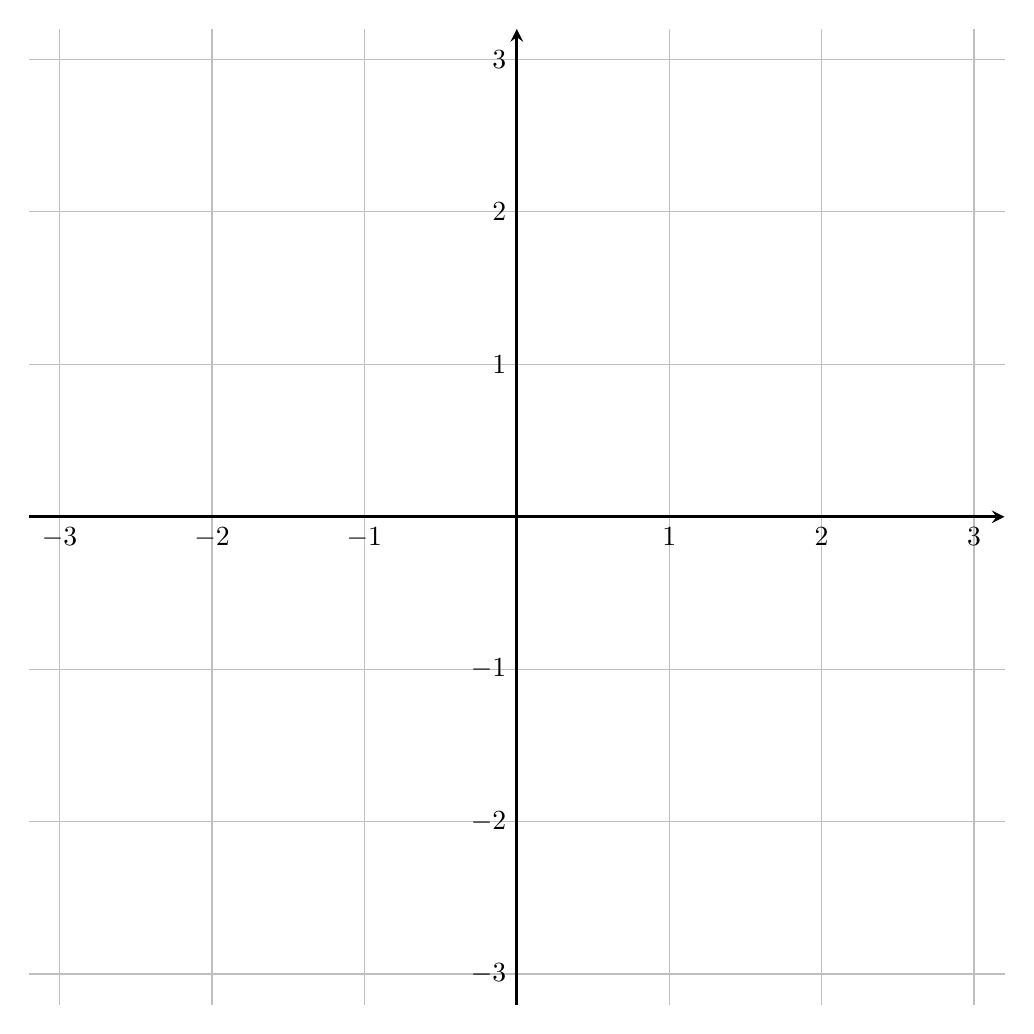
\begin{tikzpicture}
\begin{axis}[thick,smooth,no markers,
        xmin=-3.2, xmax=3.2,
        ymin=-3.2, ymax=3.2,
        xtick={-3,...,3},  
        % xticklabels= {,,},
        ytick={-3,...,3},
        % yticklabels= {,,},
        major tick length={0},
        line width=1pt,
        axis lines=center, height=5.5in, width = 5.5in, grid=major]
        % \addplot [domain=-3.2:-0.01, samples=100, name path=f, thick, color=black!50]
        % {((x-1)^2)/(2*x^2)} ;
        % \addplot [domain=0.01:3.2, samples=100, name path=f, thick, color=black!50]
        % {((x-1)^2)/(2*x^2)} ;
\end{axis}
\end{tikzpicture}
\vspace{1.5in}
\end{center}

\pagebreak

\question $\ $

\begin{parts}
    \part[10]
    Show that the equation $8x + 4\sin{x} + 6 = 0$ has a root.
    \vfill
    \part
    (7 points \textbf{EXTRA CREDIT}) Show that the above equation has exactly one root.
    \vfill
\end{parts}

\pagebreak

\question[10] Find the point on the curve $y = \sqrt{x}$ that is closest to the point $(3,0)$.
\vfill

\pagebreak

\question[10] Evaluate the following
\[\frac{d}{dx} \int_{x^3}^{-5318008} \sec^7(t^3) + t \ dt.\]
\vfill
\question Evaluate the following definite integrals, if they exist.
\begin{parts}
    \part[10] $\displaystyle \int_1^5 \frac{2t}{(t^2+4)^2} \ dt$
    \vfill
    \pagebreak
    \part[10] $\displaystyle \int_0^{\pi/4} (1+\cos{\theta})^3 \sin{\theta} \ d\theta$
    \vfill
    \part[10] $\displaystyle \int_{-\pi/4}^{\pi/4} x^3 \cos^2{x} \ dx$
    \vfill
\end{parts}

\pagebreak

\question[20] Find the volume of a solid obtained by rotating the region bounded by the given curve about the specified axis.
\begin{align*}
    & y = 2x \\
    & y = x^2\\
    & \text{About the $x$-axis}
\end{align*}
\end{questions}
    
\end{document}
